% !TEX encoding = UTF-8 Unicode

\documentclass[12pt,reqno]{amsart}
\usepackage[russian]{babel}
\usepackage[utf8]{inputenc}
%\usepackage[dvips]{graphicx,graphics}
\usepackage{graphicx}
\usepackage{euscript}
\usepackage{graphics}
%\usepackage{russcorr}
\usepackage[active]{srcltx} % SRC Specials: DVI [Inverse] Search
\usepackage{amssymb,amsmath,amsthm,amsfonts}
\usepackage{amsopn}
\newtheorem{cor}{Следствие}
\newtheorem{lem}{Лемма}
\newtheorem{thm}{Теорема}
\newtheorem{prop}{Предложение}
\newtheorem*{thm_pres}{Теорема}
\theoremstyle{definition}
\newtheorem{defn}{Определение}
\newtheorem{defneq}{Эквивалентное определение}
\theoremstyle{remark}
\newtheorem*{rem}{Замечание}
\newtheorem*{deff}{Обозначение}
\usepackage{verbatim}
\usepackage{listings}
\usepackage{hyperref}
\usepackage{color}

\definecolor{dkgreen}{rgb}{0,0.6,0}
\definecolor{gray}{rgb}{0.5,0.5,0.5}
\definecolor{mauve}{rgb}{0.58,0,0.82}

\lstset{frame=tb,
  language=Java,
  aboveskip=3mm,
  belowskip=3mm,
  showstringspaces=false,
  columns=flexible,
  basicstyle={\small\ttfamily},
  numbers=none,
  numberstyle=\tiny\color{gray},
  keywordstyle=\color{blue},
  commentstyle=\color{dkgreen},
  stringstyle=\color{mauve},
  breaklines=true,
  breakatwhitespace=true,
  tabsize=3
}

\newcommand{\sug}[1]{\rule[-2mm]{0.4pt}{5mm}_{\,{#1}}}
\newcommand{\gen} {$GE^+_n(\mathbf{R}[x])\ $}
\newcommand{\genn} {$GE^+_2(\mathbf{R}[x])\ $}
\newcommand{\gn} {$G_n(\mathbf{R})\ $}
\newcommand{\gln} {$GL_n(\mathbf{R}[x])\ $}
\newcommand{\p} {\mathbf{P}}
\newcommand{\peq} {$\mathcal{P}$}
\newcommand{\po} {$\mathcal{P}_0$}
\newcommand{\ff} {$\mathbf{R}\ $}
\newcommand{\fx} {\mathbf{R}[x]}
\newcommand{\fp} {\mathbf{R_+}}
\newcommand{\fxp} {\mathbf{R_+}[x]}
\newcommand{\zx} {\mathbb{Z}[x]}
\newcommand{\zxp} {\mathbb{Z_+}[x]}
\newcommand{\basering} {$\mathbf{F}$}
\newcommand{\lfrac} [2] {\displaystyle \frac{#1}{#2}}
\newcommand{\brsum} [3] {\displaystyle \sum \limits_{#1}^{#2} \left( #3\right)}
\newcommand{\lsum} [2] {\displaystyle \sum \limits_{#1}^{#2}}
\newcommand{\br} [1] {\left( #1 \right)}
\newcommand{\tab} {\mbox{             } \quad }
\usepackage{a4wide}


\begin{document}

\section*{Описание метода Гаусса решения системы линейных уравнений}
Метод Гаусса заключается в том, что сначала нужно выписать матрицу линейной системы уравнений и столбец свободных коэффициентов справа от нее. Далее, нужно совершать элементарные преобразования строк с матрицей и такие же преобразования строк со столбцом свободных коэффициентов (элементарное преобразование -- это вычитание из одной строки другой строки, домноженной на любой коэффициент).

Метод работает тогда и только тогда, когда определитель матрицы уравнения отличен от нуля. Пусть это так. Тогда в первом столбце матрицы есть ненулевое число. Перенесем строку с этим числом на первое место, а затем из всех остальных строк, начиная со второй, вычтем первую строку с таким коэффициентом, чтобы все элементы в первом столбце, кроме первого, стали равны нулю. Далее рассмотрим подматрицу исходной матрицы, начиная со второй строки и второго столбца и применим к ней тот же алгоритм.

В итоге, матрица будет иметь верхнетреугольный вид с ненулевыми коэффициентами на диагонали. После этого, наборот, вычитаем из всех строк последнюю с таким коэффициентом, чтобы занулить все числа в последнем столбце кроме последнего. Затем, рассматриваем подматрицу исходной матрицы без последнего столбца и последней строки и применяем к ней тот же алгоритм.

В итоге, матрица будет иметь диагональный вид. Остается лишь решить систему уравнений, в которой уравнения имеют вид $k_i x_i = b_i$, и решение будет иметь вид $x_i = \lfrac{b_i}{k_i}$.

\section*{Обоснование корректности метода Гаусса решения системы линейных уравнений}

Метод Гаусса использует элементарные преобразования строк матрицы и корректен, потому что соблюдение условий $f = 0, g = 0$ равносильно соблюдению условий $f + \lambda g = 0, g = 0$.

Система уравнений преобразуется к равносильной ей системе, которая затем решается.

\section*{Условия применимости метода Гаусса для решения линейной системы уравнений}

Как уже было сказано ранее, для конструкции необходимо, чтобы определитель матрицы был отличен от нуля, иначе на очередном шаге мы не можем гарантировать, что найдем ненулевой элемент для того, чтобы за его счет обнулить все остальные в столбце.

\section*{Вычисления с тремя матрицами}

Для вычисления определителей, матричных норм и неувязок используем sage

Код программы:

%http://www.cyberforum.ru/cpp-beginners/thread102517.html
%https://ru.wikipedia.org/wiki/Число_обусловленности
\begin{lstlisting}
def get_modules_sum(numbers):
	return sum(abs(x) for x in numbers)

def get_line_modules_sum(cur_matrix):
	for line in cur_matrix:
		yield get_modules_sum(line)

def get_infty_norm(cur_matrix):
	return max(get_line_modules_sum(cur_matrix))

def get_conditionality_number(cur_matrix):
	return get_infty_norm(cur_matrix) * get_infty_norm(cur_matrix^(-1))

def elementary_transformation(cur_matrix, coefs, i, j, la):
	cur_matrix[i] -= cur_matrix[j] * float(la)
	coefs[i] -= coefs[j] * float(la)

def swap_rows(cur_matrix, coefs, i, j):
	(cur_matrix[i], cur_matrix[j]) = (cur_matrix[j], cur_matrix[i])
	(coefs[i], coefs[j]) = (coefs[j], coefs[i])

def gauss_solve(cur_matrix, coefs):
	for start_row_index in xrange(cur_matrix.nrows()):
		max_row_index = None
		max_col_value = None
		for row_index in xrange(start_row_index, cur_matrix.nrows()):
			if max_col_value == None or max_col_value < abs(cur_matrix[row_index][start_row_index]):
				max_col_value = abs(cur_matrix[row_index][start_row_index])
				max_row_index = row_index

		swap_rows(cur_matrix, coefs, start_row_index, max_row_index)

		for row_index in xrange(start_row_index + 1, cur_matrix.nrows()):
			elementary_transformation(
				cur_matrix,
				coefs,
				row_index,
				start_row_index,
				cur_matrix[row_index][start_row_index]
					/ cur_matrix[start_row_index][start_row_index]
			)

	for start_row_index in xrange(cur_matrix.nrows() - 1, -1, -1):
		for row_index in xrange(start_row_index - 1, -1, -1):
			elementary_transformation(
				cur_matrix,
				coefs,
				row_index,
				start_row_index,
				cur_matrix[row_index][start_row_index]
					/ cur_matrix[start_row_index][start_row_index]
			)

	for row_index in xrange(cur_matrix.nrows()):
		yield coefs[row_index] / cur_matrix[row_index][row_index]

def make_column(vector):
	return matrix([[x] for x in vector])

def calc_error_vector(cur_matrix, coefs, solution):
	return make_column(coefs) - cur_matrix * make_column(solution)

def calc_error(cur_matrix, coefs, solution):
	return max(line[0] for line in calc_error_vector(cur_matrix, coefs, solution))

A = matrix([[1,2,3],[2.0001,3.999,6],[15,3,6]])
B = matrix(QQ, 8, 8, lambda i, j: 1./(i + j + 1))
C = matrix([[float(10^6),float(2)],[float(10^13),float(2)]])

rows = [["det","matrix_norm","conditionality_number","error"]]
for cur_matrix in (A, B, C):
	infty_norm = get_infty_norm(cur_matrix)
	conditionality_number = get_conditionality_number(cur_matrix)
	b = list(1 for i in xrange(cur_matrix.nrows()))
	solution = list(gauss_solve(cur_matrix, b))
	error = calc_error(cur_matrix, b, solution)
	rows.append([
		float(det(cur_matrix)),
		float(infty_norm),
		float(conditionality_number),
		error,
	])
print table(rows)
\end{lstlisting}

Вывод программы:

\begin{lstlisting}
  det                 matrix_norm     conditionality_number   error
  -0.0387             24.0            72557.9534884           0.0
  2.73705011549e-33   2.71785714286   33872791095.0           9.04844199567e-09
  1.9999998e+13       1e+13           5.000001e+12            0.0
\end{lstlisting}

Вывод: точный метод Гаусса ошибается при большом числе обусловленности, а при большой норме -- не обязательно.

\section*{Описание интерполяции кубическими сплайнами}

Дан отрезок, разбитый на много маленьких отрезков. Даны значения некоторой неизвестной функции в узлах сетки. В алгоритме аппроксимации, на каждом маленьком отрезочке мы пытаемся найти кубическую функцию, которая совпадает с исходной функцией в точках сетки, при этом добавляем условия равенства первой и второй производной сосдених сплайнов в точке сетки, а также добавляем условия на то, что вторая производная в концах отрезка равна нулю.

Все условия являются линейными относительно коэффициентов всех сплайнов, поэтому формируют систему линейных уравнений, которую можно решить, и получить результирующие коэффициенты сплайнов.

\section*{Вычисления}

В качестве гладкой функции взята $x^3$, в качестве осциллирующей $\sin\left(\lfrac{1}{x}\right)$, а в качестве разрывной -- $\mathrm{sgn}(x)$.

Вот вычисляющий код:

\begin{lstlisting}
def get_segments(a, b, step):
	x = a
	while (x + step <= b):
		yield (x, x + step)
		x += step
	if x < b:
		yield (x, b)

class CubeSpline(object):
	def __init__(self, a, b, c, d, x1):
		self.a = a
		self.b = b
		self.c = c
		self.d = d
		self.x1 = x1

	def get_value(self, x):
		return self.a + self.b * (x - self.x1) + self.c/2 * (x - self.x1)**2 + self.d / 6 * (x - self.x1) ** 3

class SplineConvex(object):
	def __init__(self, func, a, b, step):
		self.splines = []
		self.segments = list(get_segments(a, b, step))
		n = len(self.segments)

		equations = [
			[1] + [0] * n,
			[0] * n + [1],
		]
		b = [
			0,
			0,
		]

		for i in xrange(1, n):
			(x_i_prev, x_i) = self.segments[i - 1]
			(x_i, x_i_post) = self.segments[i]
			f_i = func(x_i)
			f_i_post = func(x_i_post)
			f_i_prev = func(x_i_prev)
			h_i = x_i - x_i_prev
			h_i_post = x_i_post - x_i
			equations.append(
				[0] * (i - 1) + [h_i, 2 * (h_i + h_i_post), h_i_post] + [0] * (n - i - 1),
			)
			b.append(6 * ((f_i_post - f_i) / h_i_post - (f_i - f_i_prev) / h_i))

		c_coefs = list(gauss_solve(matrix(equations), b))

		for i in xrange(1, n + 1):
			c_i = c_coefs[i]
			c_i_prev = c_coefs[i - 1]
			(x_i_prev, x_i) = self.segments[i - 1]
			f_i = func(x_i)
			f_i_prev = func(x_i_prev)
			h_i = x_i - x_i_prev
			a_i = f_i
			d_i = (c_i - c_i_prev) / h_i
			b_i = (f_i - f_i_prev) / h_i + h_i * (2 * c_i + c_i_prev) / 6
			self.splines.append(CubeSpline(a_i, b_i, c_i, d_i, x_i))


	def get_value(self, x):
		for index in xrange(len(self.segments)):
			(x1, x2) = self.segments[index]
			spline = self.splines[index]
			if x1 <= x and x <= x2:
				return spline.get_value(x)



for (func, a, b, func_name) in (
	(x^3, 1., 2., "x_cubed"),
	(sgn(x), -1., 1., "sign_x"),
	(sin(1/x), 0.000001, 1., "sin_reverse_x"),
):

	g = Graphics()
	g += plot(func, (x, a, b), color='red', legend_label=func_name)
	for (step, color) in ((0.3, 'blue'), (0.05, 'green')):
		spline_convex = SplineConvex(func, a, b, step)
		g += plot(
			lambda t: spline_convex.get_value(t),
			(x, a, b), color=color,
			legend_label="{func_name}_step_{step:.2f}".format(func_name=func_name, step=float(step))
		)

	g.save("{func_name}_splines_image.png".format(func_name=func_name))

	g = Graphics()
	step = 0.05
	spline_convex = SplineConvex(func, a, b, step)
	g += plot(
		lambda t: func(t) - spline_convex.get_value(t),
		(x, a, b), color=color,
		legend_label="{func_name}_interpolation_error".format(func_name=func_name)
	)
	g.save("{func_name}_interpolation_error.png".format(func_name=func_name))
\end{lstlisting}
\newpage

\section*{Картинки}

Для функции $x^3$

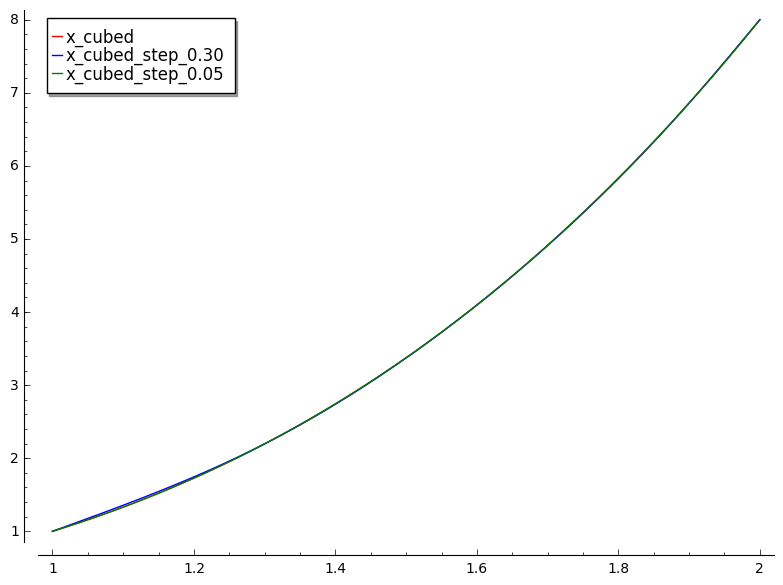
\includegraphics[width=0.4 \textwidth]{x_cubed_splines_image.png}
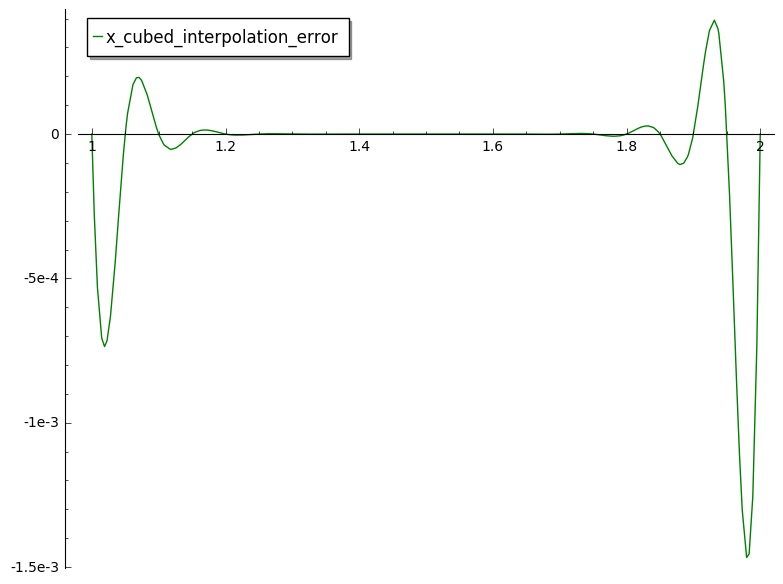
\includegraphics[width=0.4 \textwidth]{x_cubed_interpolation_error.png}

Для функции $\mathrm{sgn}(x)$

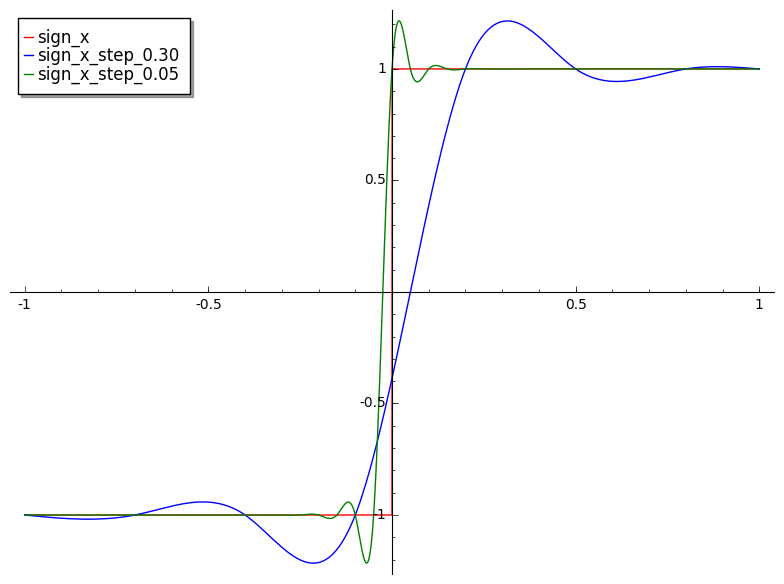
\includegraphics[width=0.4 \textwidth]{sign_x_splines_image.png}
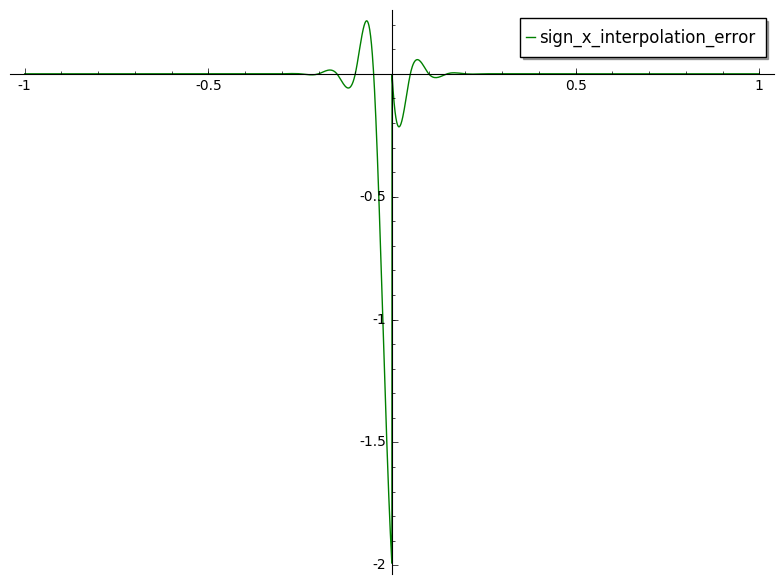
\includegraphics[width=0.4 \textwidth]{sign_x_interpolation_error.png}

Для функции $\sin\left(\lfrac{1}{x}\right)$

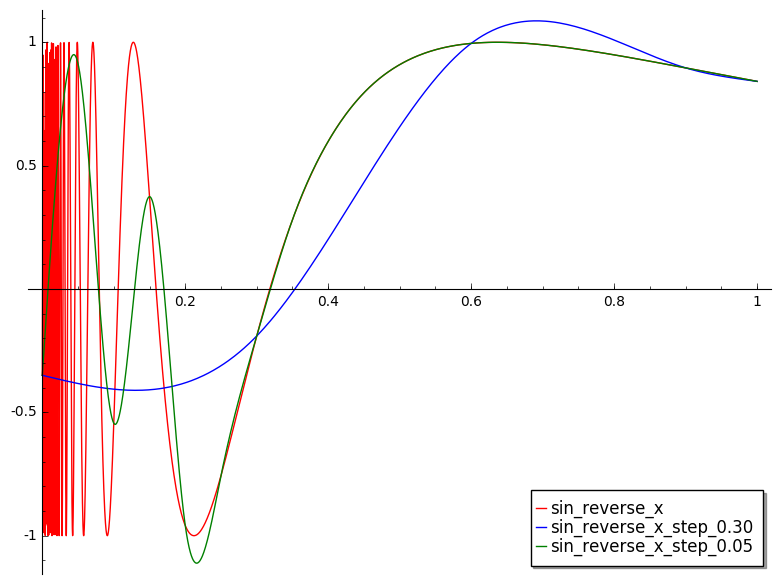
\includegraphics[width=0.4 \textwidth]{sin_reverse_x_splines_image.png}
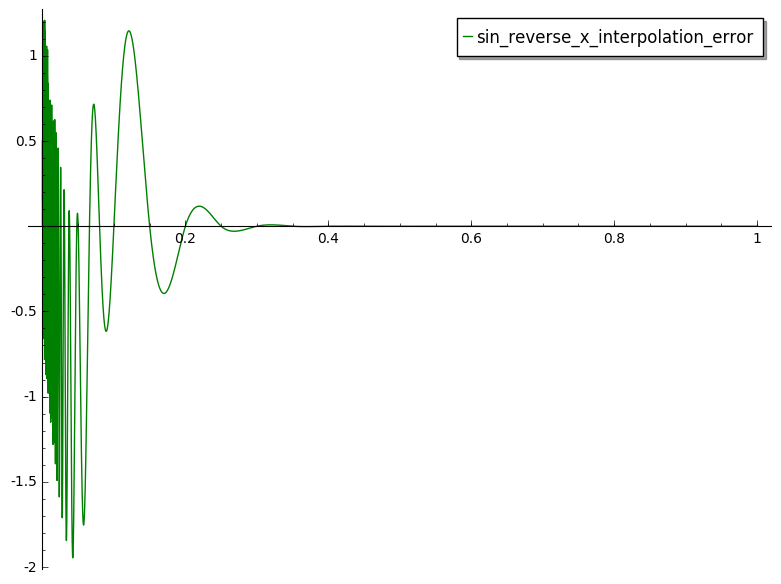
\includegraphics[width=0.4 \textwidth]{sin_reverse_x_interpolation_error.png}

\section*{Выводы про аппроксимацию}

Гладкую функцию приблизили почти идеально, но на границах приближения есть небольшие артифакты из-за того, что мы приравняли вторую производную на краях нулем, а это в реальной модели не так.

У разрывной функции наблюдаем образование лишних изгибов и экстремумов в районе разрыва.

С оцсиллирующей функцией сплайны справляются очень хорошо до тех пор, пока осцилляции не становятся в несколько раз чаще, чем шаг сетки. Но это логично, тут и невозможно ожидать более хорошего результата.

\end{document}
